% Materialer og metoder 2/5
%I dette kapitlet skal du skrive om hvordan du har gått frem metodisk, og vise hvordan valg av design og metode egner seg til å svare på problemstillingen din.

%Kapitlet må kunne gi svar på disse spørsmålene:

%Hvordan samlet du inn datamaterialet?
%Hvordan behandlet du dataene du samlet inn?
%Hvorfor valgte du disse metodene?
%Hva er styrkene og svakehetene ved disse metodene?
%Du skal også si noe om hvorfor du har gjort din undersøkelse på den måten du gjorde – og da peke på styrker og svakheter. I tillegg skal du drøfte etiske aspekter ved prosjektet. På den måten viser du at du har kommet frem til resultatene på en pålitelig og troverdig måte, men også at du er reflektert og kritisk overfor arbeidet du har gjort.

%Husk også at du her, slik som i teorikapitlet, bare skal skrive om det metodiske som er relevant for din studie.
\section{Metode}

\begin{figure}[h!]
\begin{center} 
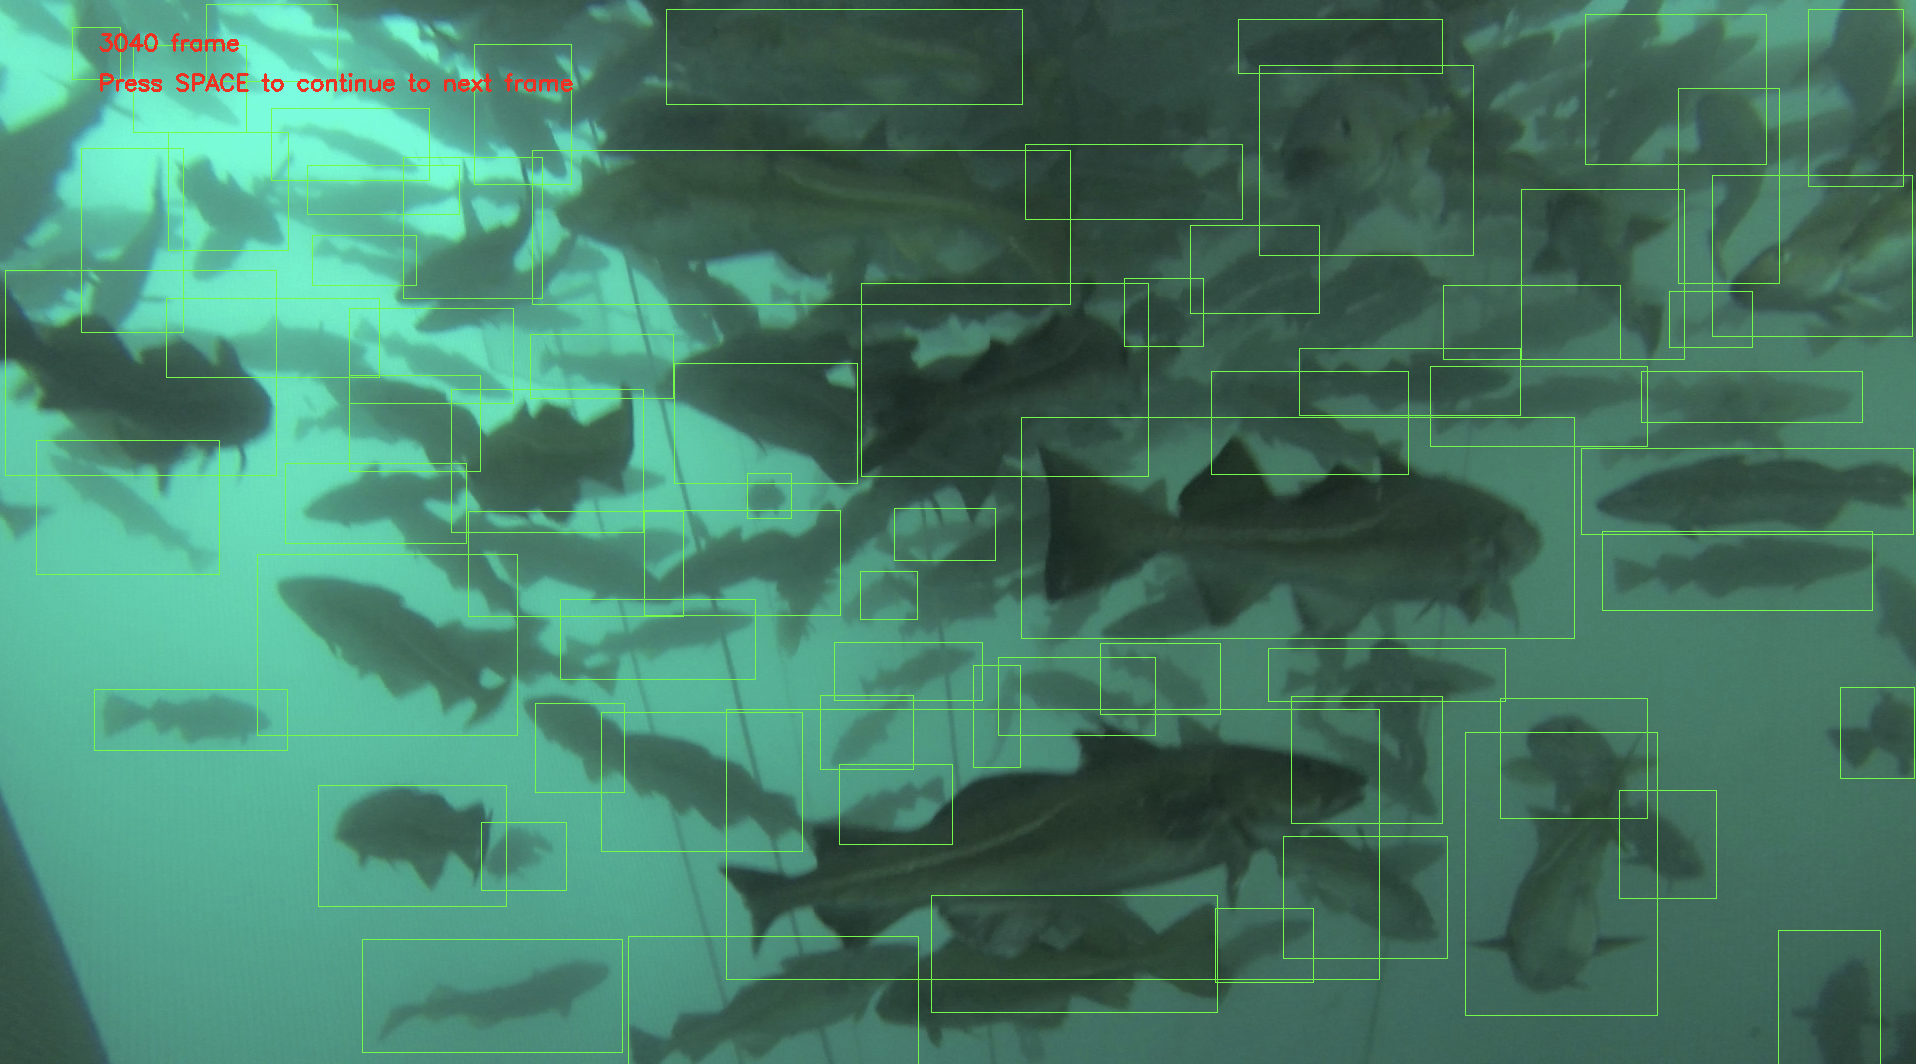
\includegraphics[scale=0.35]{figures/dataset_tool_2}
\caption{\small \sl Figuren viser et dataprogram som ble utviklet for å lage label data basert på opptakene fra Nofima. Dataprogrammet laster inn hvert femtiende bilde fra en video av en lagringsmerd av torsk. Denne videoen er 7 minutter lang. På figuren vises bilde nummer 3040. En modell som kan detektere objekter krever å bli trent på bilder av det den skal kjenne igjen, bilder med label data. Label data består av klassenummer, og $x_1$, $y_1$, $x_2$, $y_2$ posisjoner, som skaper et rektangel rundt objektene som finnes i bildet, for hvert objekt som finnes i treningsdataen. Med dette dataprogrammet så er å lage slik informasjon fra et bilde enkelt, brukeren trenger kun å lage et rektangel rundt hver torsk. Klassenummeret for torsk, her 0, og posisjonene av rektangelet, $x_1$, $y_1$, $x_2$, $y_2$, kjent som objektets ground truth bounding box, lagres til en tekstfil. Rådataen, bilde uten rektanglene eller den røde teksten som er øverst i venstre hjørne, lagres også automatisk til en mappe. \label{fig:dataset_tool}} 
\end{center} 
\end{figure} 

%Dette kapitlet er obligatorisk for alle forsøksoppgaver. Det bør innledes med et flytskjema/oversikt og en beskrivelse som letter leserens forståelse av hva som er gjort. Dette gjelder både for rene analyseoppgaver og for produktutviklingsoppgaver. 

%Beskrivelsen av materialer og metoder skal være tilstrekkelig detaljert slik at andre kan vurdere arbeidet og om ønskelig gjenta forsøkene. Samtidig må man unngå å fylle opp rapporten med unødige detaljer. Dersom det er brukt en velkjent metode, er det nok å bruke metodens offisielle navn og henvise til offisiell kilde. Hvis det var nødvendig med modifikasjoner eller andre tilpasninger i forhold til metoden, må dette beskrives. Eventuell teori om metoden, hører hjemme i teoridelen. Beskriv det dere har gjort og ikke det dere skulle ha gjort. 

%Hensikten med kapitlet Materialer og metoder er at andre skal kunne utføre det samme arbeidet på samme måte. Da må alle nødvendige opplysninger være med.

Trening av kunstige nevrale nettverk gjøres i seks steg. Det ble trent opp to modeller, en RetinaNet modell og en YOLOv3 modell. Nettverkene hadde forhåndstrente vekter fra en modell trent på COCO datasettet til Microsoft, de ble ikke trent fra scratch. %You should design a model which achieves 85 \% validation accuracy on the given dataset.

Microsoft Azure plattformen ble anvendt til å trene modellene. Microsoft tilbyr Nvidia Titan GPU-er i skyen, det gjør at treningen kan utføres uten at en trenger å investere i mektige grafikkprosessorer, store mengder datakraft blir tilgjengelig for folk flest. Å anvende GPU-er når en trener kunstige nevrale nettverk gjør at treningen tar mindre tid. Det tok ca. 2 dager å trene YOLOv3 modellen på nettskyen Azure med maskinstørrelsen Standard NC6 Promo (6 vcpu-er, 56 GiB dataminne). Trening av RetinaNet tok mye mindre tid, men inferens av RetinaNet tok over seks timer for 7 minutter video. YOLOv3 kan gjøre inferens på noen millisekunder per bilde, der RetinaNet bruker titals sekunder selv på kraftig maskinvare.% Se figur retinanet vs yolov3 resultater

\subsection{Å forstå problemet}

Før en begynner så er det viktig å være sikker på at man forstår problemet en skal løse. I denne oppgaven så skulle mengden av to fisk, torsk og sei, telles. Det er to klasser. For å løse denne oppgaven kreves bilder av hver fisk med korrekt label-data og et rimelig stort nettverk som kan forstå og trenes på bilder.

Objektdeteksjon handler om to ting. Områder av bilde som kan inneholde en klasse må genereres, og så må disse delene av et bilde klassifiseres basert på det visuelle innholdet i bildeområdet, et bildeområde kalles for en patch innenfor maskinsyn. Områdene der det kan være objekter kalles for ankre. Med andre ord, målet for modellen er å se på en del av et bilde og finne ut hvilket objekt som finnes i dette området. Nettverket kan kun finne de objektene som den har blitt trent til å gjenkjenne.

\subsection{Få tak i data}

Det neste steget var å få tak i data. Datasettet som ble laget for dette prosjektet bestod av bilder fra en lagringsmerd av torsk, og bilder av torsk og sei fra under et oppdrettsanlegg. Bildene er basert på opptak fra Nofima. Se figur \ref{fig:data}. Opptakene ble omgjort til bilder, og label data lagt inn manuelt. Se figur \ref{fig:dataset_tool}. Dette er fargebilder, så de består av tre kanaler, og har størrelsen 1920 $\times$ 1080. %You need to achieve 85 \% accuracy for validation data to successfully complete this assignment. Check it out here.

Datasettet bestod av 208 bilder av torsk, med til sammen 4582 instanser av torsk i bildene. Det var (--) bilder av sei med (--) instanser av fisken i bildene. Bildene av torsk og sei ble satt i hver sin mappe. De ble splittet etter forholdet 80/20, 80 \% av dataen var for trening, og 20 \% for validering.

\subsubsection{Utforsk og forstå dataen}

Det er viktig å se på dataen før en begynner å trene et nettverk. Det er viktig å se etter bias i bildene. Det er lurt å gå igjennom hvert eneste bilde, og se om det er noe en kan lære. Torsk og sei bildene kunne bli augmented, de kunne blant annet bli snudd horisontalt. Det gir dobbelt så mye treningsdata. Vær obs på at ikke alle treningssett tillater dette, for eksempel et datasett med lego.

Det finnes to klasser i datasettet, torsk og sei. Se figur \ref{fig:tree} og tabell \ref{tab:classes}.

\begin{figure}[h!]
\Tree[.Datasett [.labels ] [.train [.atlantic\_cod ]
               [.saithe ]]
          [.validation [.atlantic\_cod ]
                [.saithe ]]]
\caption{\small \sl Figuren viser et tre av mappestrukturen til datasettet. \label{fig:tree}} 
\end{figure} 

\begin{table}[h!]
\bigskip
\centering
\caption{Klassenavn og navneenkoding for datasettet}
\label{tab:classes} 
\begin{tabular}[t]{lcc}
\toprule
Klassekode & Klassenavn    & Norsk klassenavn \\
\midrule
0          & atlantic\_cod & torsk            \\
1          & saithe        & sei         \\
\bottomrule	
\end{tabular}
\end{table}

`Labels` mappen inneholder bounding box data for bildene. Det er en eller flere linjer per `.txt` fil. Hver linje representerer en bounding box. Representasjonen er i `xmin`, `ymin`, `xmax`, og `ymax` formatet. Se tabell \ref{tab:bbox}.

\begin{table}
\bigskip
\centering
\caption{Label data for bilde \url{Datasett/train/atlantic_cod/fish_9440.png}, lagt i fil \url{Datasett/labels/fish_9440.txt}}
\label{tab:bbox} 
\begin{tabular}[t]{lcccc}
\toprule
Klassekode    & xmin      & ymin    & xmax     & ymax \\
\midrule
0 & 238 & 643 & 582 & 882 \\
0 & 80   & 858 & 368 & 1071 \\
\bottomrule	
\end{tabular}
\end{table}

\subsection{Gjør klar dataen}

Da dataen hadde blitt organisert, og label data nøye konstruert, så ble nettverkene konfigurert og treningen ble satt i gang. Dataen ble matet inn i treningsprogrammet, inn i deep learning rammeverkene.

Det ble trent opp to nettverk. Den ene, RetinaNet, er en del av detectron2 fra Facebook. Den ble trent og konfigurert med PyTorch. Den andre modellen var YOLOv3, den er utviklet av Joseph Redmon og trenes med deep learning rammeverket som han har skrevet i C, den heter darknet. Konfigurasjon gjøres ved å endre på tekstfiler og kommandolinjeparameterene til rammeverket.

\subsubsection{Dataaugmentering}

Dataen må først normaliseres på en standard måte, for eksempel ved å subtrahere gjennomsnittet over dataen, for så å skalere alle bildene slik at de får samme størrelse. Det er også mulig å gjøre flere andre endringer. Støy kan legges til bildene, samt å snu dem horisontalt eller vertikalt for å skape nye bilder å trene nettverket på.

Det ble ikke gjort endringer på standardmåten detectron2 og darknet gjør dataaugmentering.

\subsubsection{YOLOv3 label data og bildeformat}

YOLOv3 har et annet label-format sammenlignet med RetinaNet, dessuten krever den bilder i jpeg formatet, med filudvidelsen .jpg. Label-dataen legges sammen med bildene. Konvertering fra RetinaNet sitt format til YOLOv3 ble gjort med et awk-skript. Formatet til YOLOv3 er:

\begin{verbatim}
[klassenavn] [objekt midtpunkt i X] [objekt midtpunkt i Y]
	[objekt vidde i X] [objekt høyde i Y]
\end{verbatim}

Et nyttig verktøy til å konvertere bilder er John Cristy sin Image Magick. Her er hvordan bildene ble konvertert fra Adobe sitt png format til jpeg:

\begin{verbatim}
mogrify -format jpg *.png
\end{verbatim}

\subsection{Tren nettverket på et lite utvalg av dataen som en test før en trener et fullt nettverk}

Nettverket ble først trent opp på et utvalg av treningsdataen, for å teste nettverket. 208 bilder med 4582 instanser av torsk ble grunnlaget for de første RetinaNet og YOLOv3 modellene.

RetinaNet modellen ble trent med en learning rate på 0,001 over 500 iterasjoner. Modellen brukte vekter fra COCO, den ble lastet ned fra the model zoo, den heter \url{COCO-Detection/retinanet_R_50_FPN_3x.yam}. RetinaNet sin score threshold ble satt til 0,5. Batch size var 4.

Define configurations in the section — a configuration like training configuration, system configuration. In the section, you can define batch size, data path, learning rate, etc.

You need to set up the training pipeline with a batchsize of 4 and run the experiment for 100 epochs. Make these changes in the Configrations given below.

\subsection{Trene modellen på hele datasettet}

Optimizers and learning rate schedulers [You can even get good results without a learning rate shceduler]
Regularization techniques like Data Augmentation, Dropout, BatchNorm

\subsection{Forbedre modellen}

Lowering learning rate helps
Adding a convolutional layer helps
Increasing epochs helps when learning rate is low
Decreasing batch size ...

\subsection{Inferens}

You only look once (YOLO) er en state-of-the-art, real-time objektdeteksjonssystem. På en Pascal Titan X, en mektig Nvidia GPU, så prosesserer den bilder ved 30 FPS har har en mAP på 57.9 \% på COCO test-dev \cite{Redmon m.fl. 2020}. På min Macbook Pro fra 2017 så drar den 1 FPS på CPU-en på datasettet presentert i denne oppdaven. Ifølge Redmon så er YOLOv3 like bra som Focal Loss, det er RetinaNet, men omtrent fire ganger raskere. Min erfaring er at den er rundt 10 ganger raskere, men mye mindre nøyaktig (må gjøre et eksperiment her). Redmon mener en kan lett endre størrelsen på YOLO modellen, den vil bli tregere men enda mer nøyaktig \cite{Redmon 2020}. Se figur \ref{fig:yolo_inference}, \ref{fig:retinenet_inference} og \ref{fig:inference}.

\begin{figure}
\begin{center} 
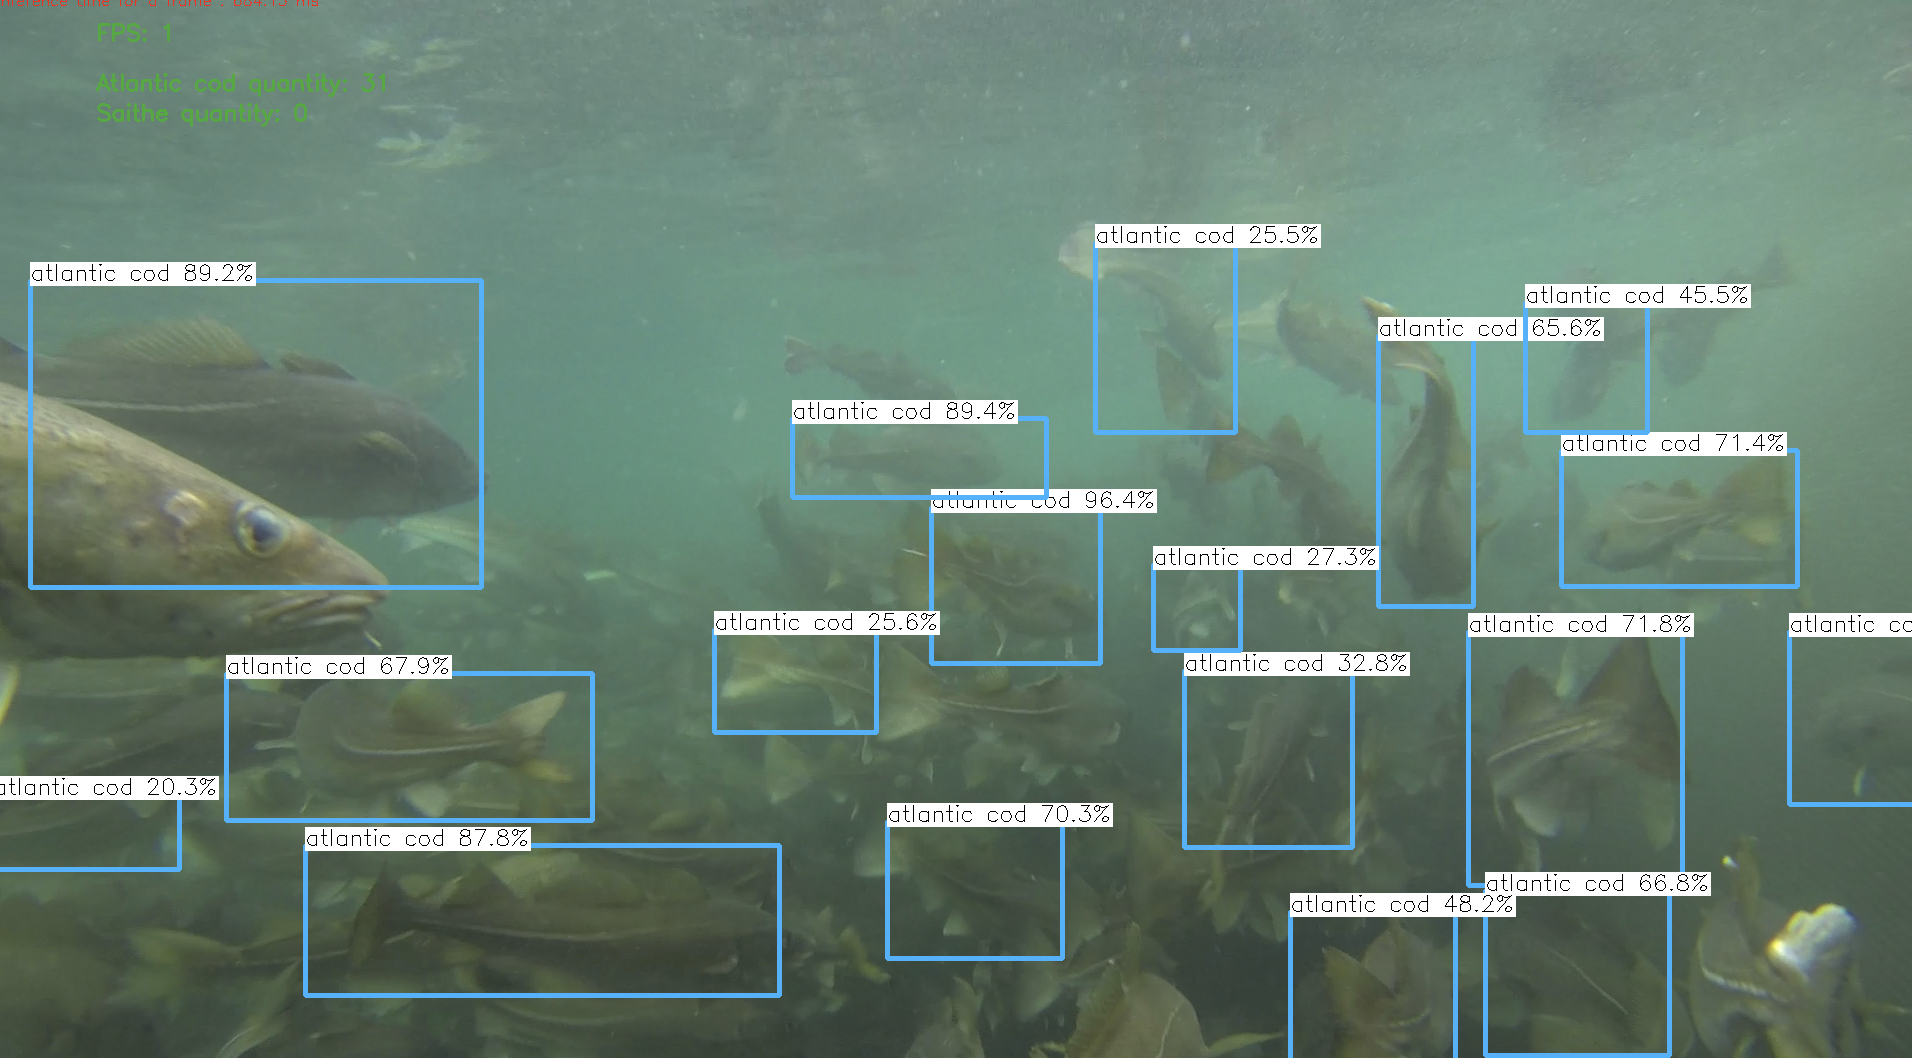
\includegraphics[scale=0.35]{figures/inference_yolo}
\caption{\small \sl Figuren viser inference med YOLOv3. Rundt fiskene så lager YOLOv3 bounding boxes der den tror det finnes fisk, og gir den en label basert på det den tror at det er. Her får alle fiskene labelen ``atlantic cod'', dette er fra en lagringsmerd med torsk. Ved siden av navnet av klassen så står det hvor sikker nettverket er på at den har funnet en torsk, presisjonen av inferensen. I grønn tekst, øverst til venstre, står det at algoritmen kan telle 31 torsk i bildet, og 0 sei. \label{fig:yolo_inference}} 
\end{center} 
\end{figure} 

\begin{figure}
\begin{center} 
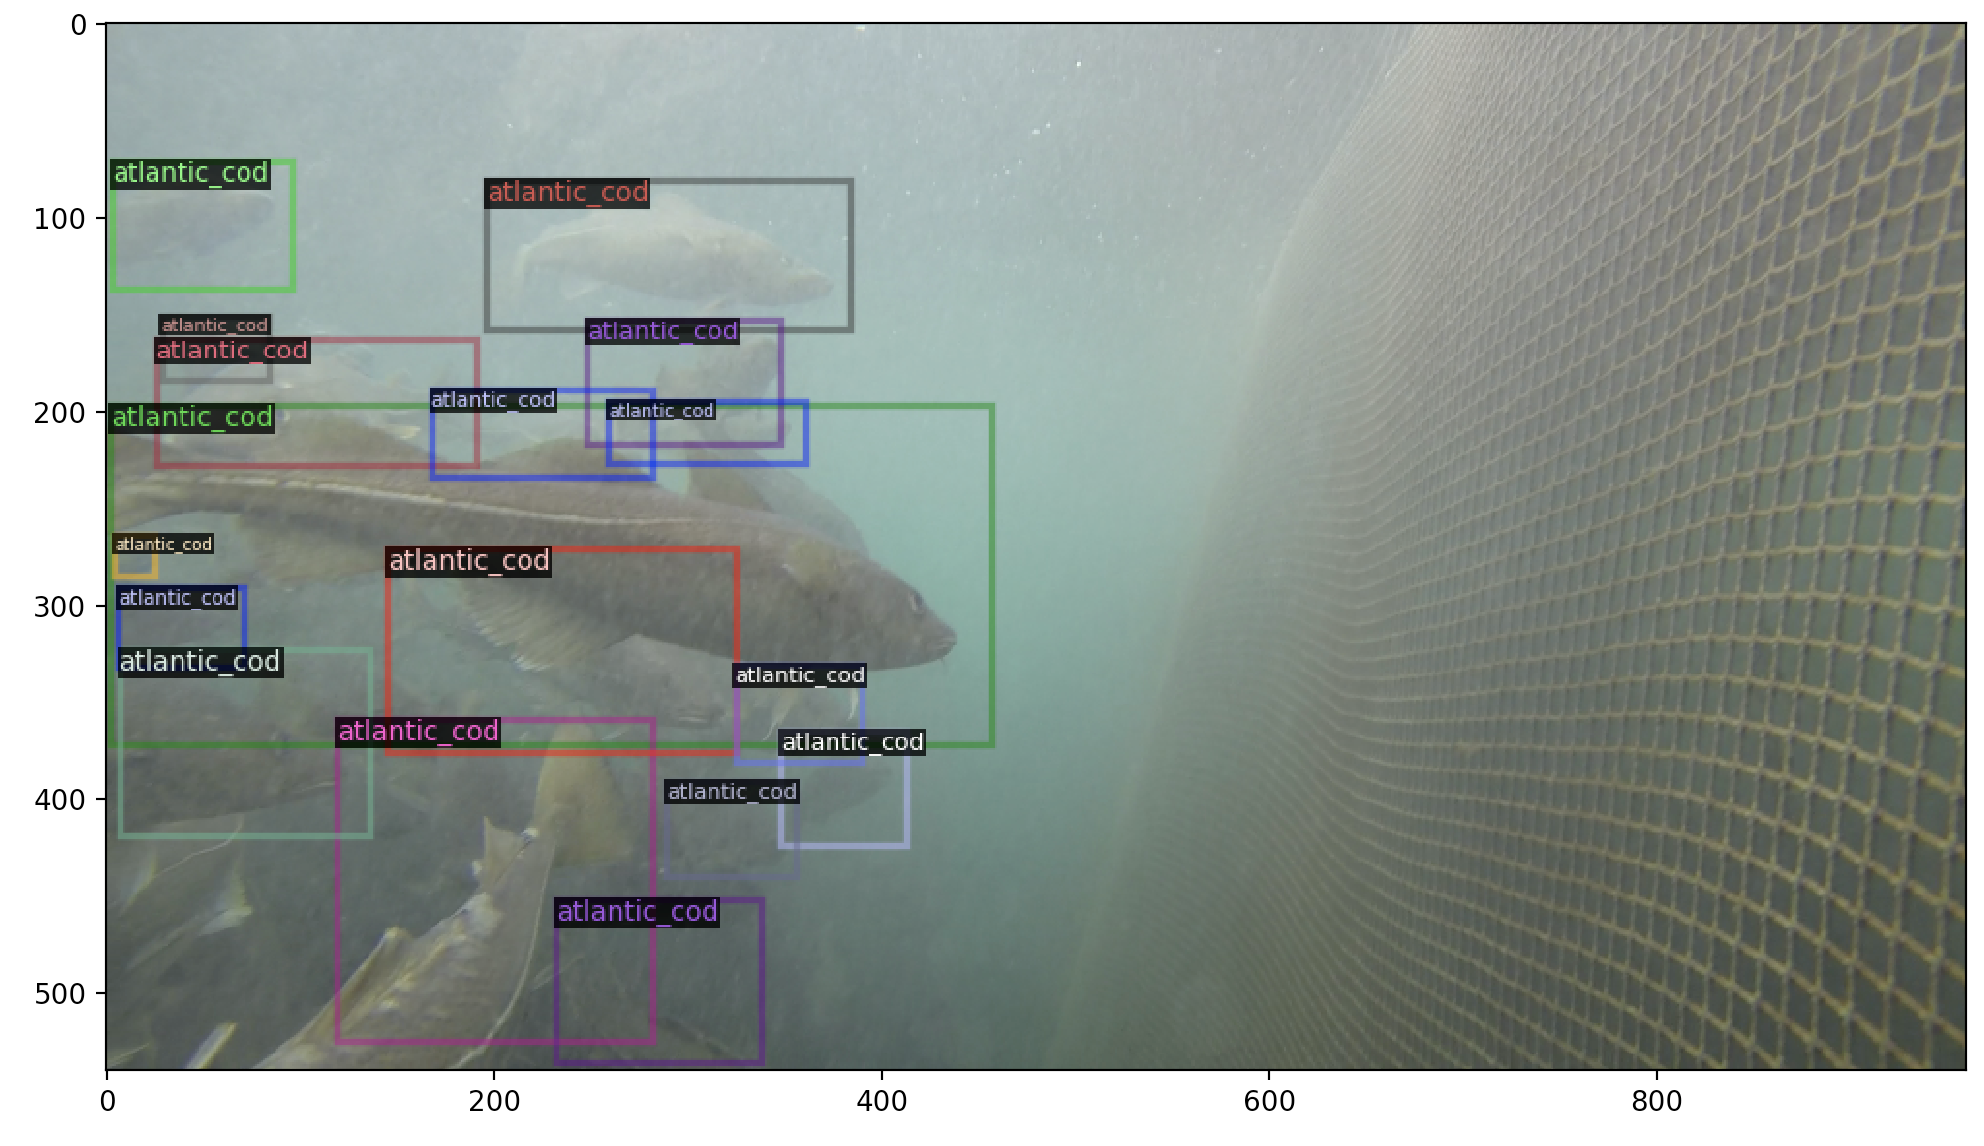
\includegraphics[scale=0.35]{figures/retinanet_cod}
\caption{\small \sl Figuren viser inference med RetinaNet. \label{fig:retinenet_inference}} 
\end{center} 
\end{figure} 

\subsubsection{OpenCV program}

%\subsection{COCO Detection Evaluation} % For analyse kapittelet?
